\documentclass[conference]{IEEEtran}
\usepackage[noadjust]{cite}
\usepackage[utf8x]{inputenc}
\usepackage[english]{babel}
\usepackage[nottoc]{tocbibind}
\usepackage{graphicx}
\usepackage{nameref}
\usepackage[hidelinks]{hyperref}
\usepackage{sidecap}
\usepackage{wrapfig}
\usepackage[bottom,hang]{footmisc} 
\usepackage{acronym}
\usepackage{color}
\usepackage{afterpage,hyperref} 
\usepackage{listings}
\usepackage{subfigure}
\usepackage{array,			%better tables
			tabularx,			    %instead of tabular*             
			booktabs,			%tables for good publications
}

\begin{document}
\title{Seminar on Privacy in Ubiquitous Computing}

\author{\IEEEauthorblockN{Mehmed Mustafa}
\IEEEauthorblockA{\textit{Institute of Computer Science} \\
\textit{University of Göttingen}\\
mehmed.mustafa@stud.uni-goettingen.de}
\and
\IEEEauthorblockN{Chris Warin}
\IEEEauthorblockA{\textit{Institute of Computer Science} \\
\textit{University of Göttingen}\\
chris.warin@stud.uni-goettingen.de
}
}

\maketitle

\begin{abstract}
This document is a model and instructions for \LaTeX.
This and the IEEEtran.cls file define the components of your paper [title, text, heads, etc.]. *CRITICAL: Do Not Use Symbols, Special Characters, Footnotes, 
or Math in Paper Title or Abstract.
\end{abstract}

\begin{IEEEkeywords}
privacy, bystander, privacy enhancing technology
\end{IEEEkeywords}

\section{Introduction}
Today's society is filled with technological devices that are capable of gathering data from people, such as smartphones, surveillance cameras, \ac{AR} devices or \ac{IoT} devices \cite{lu2017privacy, shu2016cardea, denning2014situ}. Although these devices have been causing a number of concerns regarding the privacy of users, recent studies have shown that the privacy of bystanders (i.e. the individuals that are around users using these devices) is also often involved, as online-shared data often involves individuals other than the users sharing the data~\cite{olteanu2018consensual}. In other words, bystanders' personal information can be collected without their knowledge or consent~\cite{lu2017privacy}.

A common real-life example could be a person taking a picture in a busy street, where the faces of bystanders are recognizable. The picture can later be posted on social media, and neither the posting or the taken picture have been made with the knowledge nor consent of the bystanders \cite{shu2016cardea}. This example can easily be adapted with different mediums (i.e. pictures, videos, audio), and the collected data can be of different nature (i.e. face, voice, location). This high amount of devices capable of collecting data of different nature results in high pervasiveness in bystanders' privacy. This is a significantly harder problem to solve than regular user privacy, mainly because bystanders can be unaware that data involving them is shared in the first place~\cite{olteanu2018consensual}.

In the past, several attempts with different approaches have been made in order to ensure the privacy of bystanders. Technological solutions exist: for visual privacy, Gaussian blur, pixelisation \cite{dufaux2010framework} have been used in order to anonymize individuals---this is most commonly seen on TV. Olteanu, Huguenin, Dacosta and Hubaux~\cite{olteanu2018consensual} claim that few solutions exist for detecting and sharing interdependent data in a consensual and privacy-preserving way. Legal solutions have also been applied (e.g. forbidding the use of cameras, smartphones, or \ac{AR} devices like Google Glass in certain places\cite{shu2016cardea}). However, these have been proven either inefficient or insufficient~\cite{shu2016cardea, olteanu2018consensual, dufaux2010framework}. 

Due to the inefficient past attempts to ensure bystanders' privacy, the issue remains to be solved. There can however not be a perfect solution, because of several critical aspects. First, individuals have different requirements in terms of privacy, and these requirements can change over their life~\cite{shu2016cardea}. According to Westin~\cite{langheinrich2009privacy}, they are categorized between privacy fundamentalists (i.e. distrustful regarding organizations requiring their data), pragmatics (i.e. deciding whether they want to obtain various services, opportunities, and more, in exchange of the potential pervasiveness caused by the organisation's information seeking), and unconcerned (i.e. trustful regarding organisations requiring their data). Although this categorization concerns the privacy requirements of individuals, the same can be applied when they become bystanders to the eye of others. In consequence, fundamentalists will seek solutions that will, for example, systematically anonymize them to ensure their privacy as bystanders. Pragmatists will decide whether they want to adopt a certain solution depending on certain aspects (e.g. the cost, how good the solution protects them, the usability of the solution) and with varying requirements in privacy (e.g. decide to not be anonymized to trusted users). Unconcerned will remain unaware of having their privacy compromised, or will not want to adopt a privacy enhancing solution because of the added complexity. This means that there cannot be one solution to fit everyone. Moreover, because bystanders can be unaware of being present in other individuals' data, most solutions require that they register themselves on the system to define their preferences. In other words, very few solutions can enhance the privacy of bystanders such that they don't need to care or take action about it.

%new solutions

%we have defined our topic, selected papers based on XYZ, refined the selection based on the following criteria. As a result, we compare XYZ solutions organised around XYZ

The protection of bystanders' privacy is a concern that touches several domains, namely economical, social, legal, and technological~\cite{lu2017privacy}. This report focuses on the different technologies that address the pervasiveness in the privacy of bystanders. Section~\ref{BystandersPrivacy} lists different real-life examples of bystanders' privacy being compromised. Section~\ref{Technologies} goes over different technologies that ensure different aspects of the privacy of bystanders. Section~\ref{Limitations} describes the current limitations and challenges that these technologies are facing, whether they are technological or not. Finally, section~\ref{Conclusion} concludes this report.

\section{Bystanders’ privacy pervasiveness}\label{BystandersPrivacy}
Give real-life examples and why they are problematic.
\subsection{Videos and images}
Surveillance cameras, smartphone photos/videos in the street capturing bystanders
\subsection{Audio}
Google Home / Amazon Alexa in a household: other members are also listened
\subsection{Location}
Pervasive location information in apps (e.g. French StopCovid app recenses more contacts’ location information than announced)
\subsection{Others}
IoT, see example in 2.b

\section{Technologies for ensuring the privacy of bystanders}\label{Technologies}

\subsection{PriSurv System}
Video surveillance systems are necessary for a safe and secure community, which explains why they are widely deployed. However, high deployment rate of these systems in public places leads to privacy invasion of the objects being recorded. Solution of this problem is a challenging task because privacy and security should be balanced appropriately and when possible in real-time.

There are several other studies on privacy based on video surveillance. Two studies proposed image processing methods in order to protect the privacy of objects \cite{cavallaro2005},\cite{kitahara2004}. In other two studies the privacy protection of objects depends either on the authority of objects or observers \cite{jehan2005},\cite{senior2005}. Privacy information can be embedded by using digital watermarking technology in such way that only predefined authorized viewers will have access to it \cite{zhang2005}. However, these solutions are not flexible enough, because the sense of privacy of different objects is not considered. For example, object A may want their privacy to be protected from observer A, but not from observer B. Some objects may not want a privacy protection at all. 

PriSurv system \cite{chinomi2008PriSurv} can adaptively protect privacy of objects and disclose their visual information according to the privacy policies of the different objects. PriSurv is a video surveillance system, which is defined by visual abstraction and protects the privacy of objects appearing within a video depending who observes the video. Closeness between objects and observers determines the privacy policies to be used. 


\subsubsection{Simple run case}

\begin{figure}[t]
\centerline{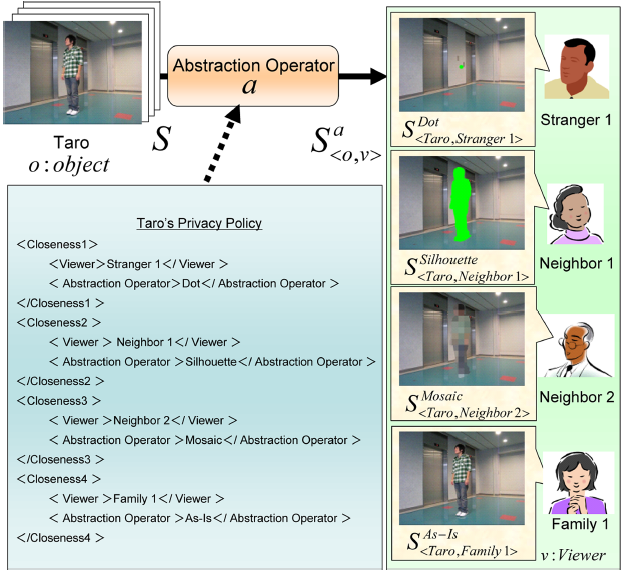
\includegraphics[width=.5\textwidth]{img//prisurv_simple_demo.png}}
\caption{PriSurv simple run case \cite{chinomi2008PriSurv}.}
\label{fig:prisurv}
\end{figure}

Figure~\ref{fig:prisurv} is an example run case of PriSurv, which shows how visual abstraction is used in order to protect the privacy of an object appearing within an image. Let o, a, v and S denote an object, an abstraction operator, a viewer and an original image, respectively. In the example, “Taro” is the object which appears within the original image and is monitored by “Stranger 1”, “Neighbor 1”, “Neighbor 2” and “Family 1” which are the different viewers. Since the closeness between the object and viewers is different, different abstraction operators are used for hiding the visual information of the object. In the example, these operators are “Dot”, “Silhouette”, “Mosaic” and “As-Is”, which are 4 of the 12 possible operators. Each viewer then receives a privacy protected version of the original image which is denoted by $S_{<o, v>}^a$. A simplified version of Taro’s privacy policy, which is a part of the abstraction operator, is also available to give a better understanding of how the closeness is defined. 

\subsubsection{System overview}

\begin{figure}[t]
\centerline{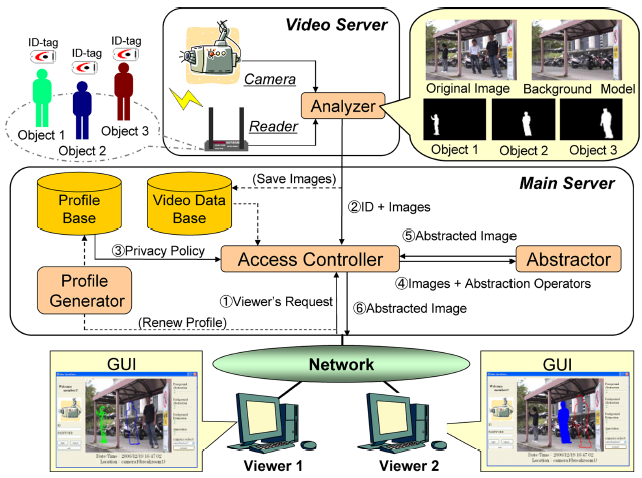
\includegraphics[width=.5\textwidth]{img//prisurv_arch.png}}
\caption{PriSurv system overview \cite{chinomi2008PriSurv}.}
\label{fig:prisurv2}
\end{figure}

Figure~\ref{fig:prisurv2} shows the architecture of the PriSurv system. It consists of three main parts: Video Server, Main Server and Network. It also has six different components: Analyzer, Profile Generator, Profile Base, Access Controller, Abstractor and Video Data Base. 

The Analyzer, which is a part of the video server, is responsible for identifying different objects. Each identifiable object must have its own \ac{RFID}-tag. The surveillance area is divided into smaller N x N areas and the location area of each \ac{RFID}-tag is determined by an \ac{RFID}-reader. Each object inside the original image is extracted and then identified separately by comparing the obtained visual data with the binary images of each object. 

The Profile Generator is used for setting up privacy policies for different members of the system. Each member's personal information such as name, age, gender and address and privacy policy is stored securely inside the Profile Base. The Profile Generator is also responsible for converting data taken from the GUI to \ac{XML}-based syntax. The profile of each member can only be updated by them and other members have no access to this data. 

The Access Controller determines the closeness relationship between a requesting viewer and an object to be monitored by reading the \ac{XML}-based privacy policies of the object stored inside the Profile Base. Once the types of abstraction operators are extracted, Access Controller sends them to the Abstractor. 

The Abstractor is a processor for images that performs visual abstraction by using abstraction operators. 

The Video Data Base stores past video data and makes it available to viewers after appropriate visual abstractions are performed. 

\subsection{Cardea Framework}

Surveillance cameras are not the only threat for the visual privacy of people. Availability of cameras within modern mobile and wearable devices has also increased people's concerns about their visual privacy, because nowadays taking photos or recording videos and then sharing online is easier. Moreover, sharing pictures and videos online could reveal more information than expected, especially when the data is publicly available. Usage of recognition technologies which are able to correlate the shared data to specific people, places, and things, could make the data searchable \cite{gross2014},\cite{shaw2006}. Even when taking photos is not involved, applications making use of the camera, such as \ac{AR} apps, could still compromise the visual privacy of bystanders by leaking the captured visuals, maliciously or not. 

Privacy issues raised by unnoticed or unauthorized collection of visuals have been addressed, both legally and technically. Google Glass, for instance, is not allowed to be used at places such as hospitals, bars, and movie theatres [footnote 3]. However, banning such devices is not a good and fundamental solution, because it takes away the possibility of people to capture and share happy moments, especially if there are not any bystanders around. As a result, there are increasing needs to design technical solutions which can protect visual privacy of individuals while not restricting the rights of other individuals. 
	
There are proposals for using visual markers \cite{roesner2014},\cite{liu2014} or colourful hats \cite{sastry2007} with which people can declare their disagreement to be captured. These approaches, however, are not flexible enough, because people should be able to control, modify and express their individual privacy preferences naturally – without the need of any extra facilities. PriSurv system, which was discussed in the previous section, also relies on extra facilities such as \ac{RFID}-tags and -readers. Thus, it is not a feasible solution for built-in cameras. 

The Cardea framework \cite{shu2016cardea} does not rely on such or similar extra facilities, instead it takes advantage of computer vision techniques which are effective and reliable. Moreover, it allows people to change their privacy preferences dynamically, for example, by using predefined hand gestures. The framework also specifies context elements, such as scenes and presence of others. People can set their personal privacy profiles, hand gestures for flexible interaction with cameras and define context related privacy preferences. For example, some people might prefer their visual appearance to be hidden inside bars, but not in the parks. But in cases when they prefer to appear in photos, taken inside a bar, they can enable it with a hand gesture. Devices using the framework will automatically compute factors related to context, check people's privacy preferences, and protect their visual appearance by blurring their face.


\subsubsection{Framework Overview}
\begin{figure}[t]
\centerline{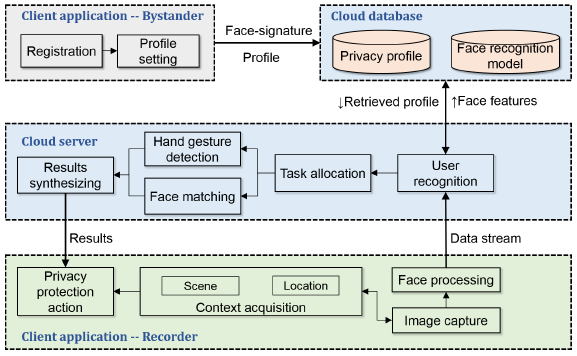
\includegraphics[width=.5\textwidth]{img/cardea_overview_diagram.png}}
\caption{Cardea framework overview \cite{shu2016cardea}.}
\label{fig:cardea2}
\end{figure}

Frame overview will be here 



\subsubsection{Example run case}
\begin{figure}[t]
\centerline{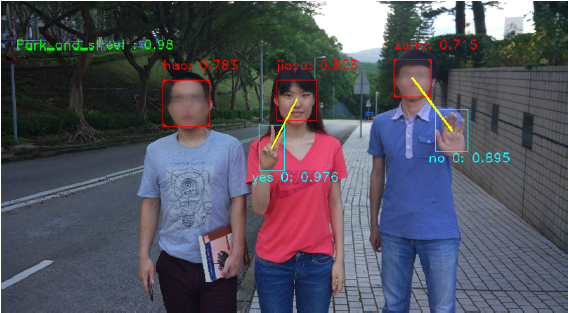
\includegraphics[width=.5\textwidth]{img/cardea_example.png}}
\caption{Cardea framework example run case \cite{shu2016cardea}.}
\label{fig:cardea}
\end{figure}

Example run case will be here 



\subsection{Sharing of Multi-Subject and Interdependent Data}
Reference \cite{olteanu2018consensual}


\subsection{Others - More specific Audio or Location based technologies should be found}


\section{Limitations and challenges of privacy ensuring technologies}\label{Limitations}
\subsection{Cardea (user contribution)}
Willingly putting your personal data on a cloud to avoid having your privacy invaded by others can be seen as counter productive
\subsection{Example 2}
\subsection{Example 3}
\subsection{(optionally) Ideas that could fix these limitations}

\section{Conclusion}\label{Conclusion}


\begin{table}[htbp]
\caption{Table Type Styles}
\begin{center}
\begin{tabular}{|c|c|c|c|}
\hline
\textbf{Table}&\multicolumn{3}{|c|}{\textbf{Table Column Head}} \\
\cline{2-4} 
\textbf{Head} & \textbf{\textit{Table column subhead}}& \textbf{\textit{Subhead}}& \textbf{\textit{Subhead}} \\
\hline
copy& More table copy$^{\mathrm{a}}$& &  \\
\hline
\multicolumn{4}{l}{$^{\mathrm{a}}$Sample of a Table footnote.}
\end{tabular}
\label{tab1}
\end{center}
\end{table}

\section*{Abbreviations and Acronyms}
\addcontentsline{toc}{section}{Abbreviations and Acronyms}
\begin{acronym}[Bash]
\acro{IoT} {\textit{Internet of Things}}
\acro{AR} {\textit{Augmented Reality}}
\acro{RFID} {\textit{Radio-frequency identification}}
\acro{XML} {\textit{Extensible Markup Language}}
\end{acronym}

\bibliographystyle{IEEEtran}
{\footnotesize
\bibliography{literature_list}}

\end{document}